\def\year{2017}\relax
%File: formatting-instruction.tex
\documentclass[letterpaper]{article}
\usepackage{aaai17}
\usepackage{times}
\usepackage{helvet}
\usepackage{courier}
\usepackage{graphicx}
\usepackage{booktabs}
\usepackage{diagbox}
\frenchspacing
\setlength{\pdfpagewidth}{8.5in}
\setlength{\pdfpageheight}{11in}
\setcounter{secnumdepth}{0}  
 \begin{document}
% The file aaai.sty is the style file for AAAI Press 
% proceedings, working notes, and technical reports.
%
\title{Predicting Institution Ranking: Whose paper are accepted the most}
\author{DiYi Wang, XueGuang Lu\\
Northeastern University\\
360 Huntington Ave.\\
Boston, Massachusetts 02115\\
\{wangdiyi, xueguang\}@ccs.neu.edu
}
\maketitle
\begin{abstract}
Yearly rank of Research Institution and University has become a tradition for many popular newspapers, magazines and academic publications. The impact on global advancements is an essential standard of measurement on research institutes. It forms an interesting graph in ways that outstanding scientists tend to work in influential affiliations and leading companies tend to cooperate with authoritative institutes. The topic of KDD Cup 2016 is to find influential nodes in research community. The competition convert this problem into predicting the rank of paper acceptance number by several important conferences in research field. In this paper, we show ways of improving the Ensemble Model brought by Qian and Dong[7], who was ranked overall at 2nd place in KDD Cup 2016. We improved the overall accuracy of the ensemble model and discuss ways it might be further improved in future works. All extracted feature data and source code of our model implementations are publicly available on GitHub for further research purposes [9].
\end{abstract}


\section{INTRODUCTION} 
Ranking of influential affiliations can based on several metrics: financial endowments, amount of students, amount of Nobel prized professors, location and so on. However, the main metric should be measuring the research ability of an institution. Top institutions follow the trend of advanced technologies and document their work in papers for better discussion and shared knowledge. Papers accepted by top conferences can be seen as an acknowledgment by the academic world. Therefore, we say that to measure the impact of research institutions are to measure the paper they published, by making a naive assumption that research influence is solely based on the quality and quantity of accepted papers. To further down-scope the problem, we ignore quality differences of accepted papers and weigh each accepted paper equally as recommended by competition organizer. The downside of this assumption is discussed in the Feature Engineering section.\newline


KDD Cup 2016 stands out from KDD's previous years' competitions because the ranking of affiliations is completely unknown at the time of the competition. The competition has 3 phases as the discovery of parts of the ground truth, in other words, as three conferences (SIGIR, KDD, MM) finalize their choices of 2016 accepted papers sequentially. 



\subsection{Evaluation}

Each phase is judged separately at first and then combined in the end using a weighted average of each team's NDCG@20 [2] scores at each stage. The metric of NDCG@n score is defined as follow in order to formalize a way to compare difference ranking predictions.
\begin{equation}
DCG@n = \sum_{i=1}^{n} \frac{RelavanceScore_i}{log_{2}^{i+1}}
\end{equation}
\begin{equation}
NDCG@n = \frac{DCG@n}{IDCG@n}
\end{equation}
Where $i$ is the rank of an institution, and $RelavanceScore_i$ is institution $i$ relevance score. Relevance score is calculated by scoring each paper as 1, dividing 1 by the number of co-authors and assigning the quotient to the affiliation to which the author belongs. Thus, if we suppose a paper consists of three authors from distinct universities, each university receives a score of 1/3 because of this paper.

\subsection{Dataset}
The only dataset we used, Microsoft Academic Graph (MAG)[5], is a publicly available heterogeneous graph provided by Microsoft since it is the only dataset used by other teams and is recommended by the competition organizer. The dataset contains research publications along with their associated authors, affiliations, conferences, citation relationships and field of study. The recommended snapshot of the MAG consists of 114,698,044 authors, 126,909,021 publications with 19,843 associated affiliations and conferences which we parsed, cleaned and manipulated using Python and SQLite. The features were extracted and stored into a hash map for the usage of our model implementations and possibly for other future research purposes. The feature space we extracted are of related conferences and of recent publish year; we ended up with a subset which consists of 119,425 entries. We will talk about how we process and make use of this dataset in Experiment section.\\

\subsection{Framework}
\begin{figure}[h]
    \centering
    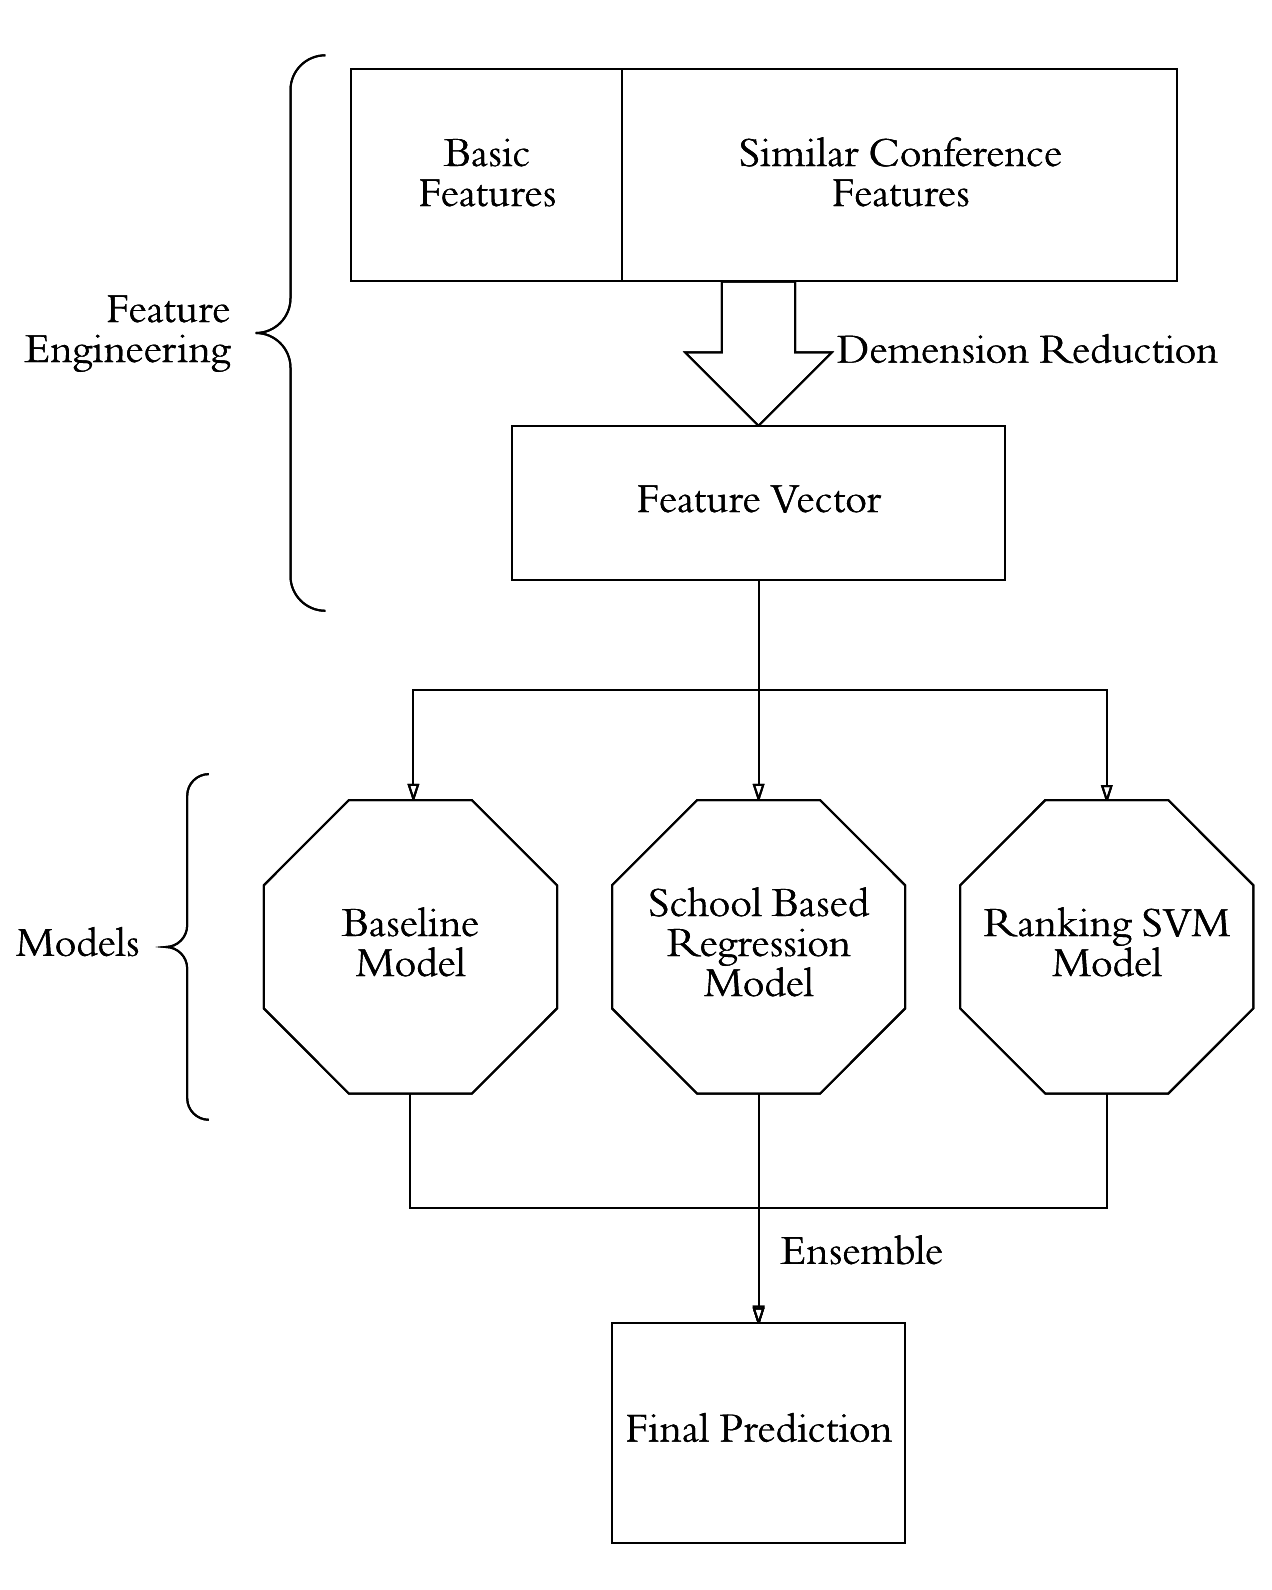
\includegraphics[width=\linewidth]{Framework.png}
    \caption{Proposed Model}
    \label{fig:my_label}
\end{figure}
As shown in Figure 1 that after feature extraction, we first reduced the dimensionality of the feature vectors in ways which are further discussed in Feature Engineering section, and supplied the reduced-dimension vector into three different models, we then compared and analyzed the results of each individual model and the ensemble model. 

\subsection{Overview}
In the following sections, we will talk about how we improved Qian and Dong's ensemble modal in Model section. Subsequently, in the Experiment section, we elaborate on 
\begin{itemize}
    \item the specifics of our dataset
    \item how we designed and utilized our model
    \item the experiment results along with their underlying rationales.
\end{itemize}
\section{RELATED WORKS}
We introduce three methods from the top 3 winners of the competition in this section. They achieved an overall score of 0.765[6], 0.758[7], 0.756[8] by using the NDCG@20 metric to measure the relevance of the ranking. Unfortunately, the organizer of KDD Cup didn't give out the test data of accepted papers in 2016. Thus, we can only compare our improved model with theirs on the existing dataset, more specifically, on the predictions of 2015 ranking using training data from 2011 - 2014.

\subsection{1st Winner}
The 1st place winner Vlad and Mihai investigated several methods on different phases of the competition. They implement Gradient boosting decision trees (GBDT) [10] on train set which contributed to finding out a new method for feature engineering. They found out who the impact of mean historical relevance is relevant to an affiliation's ranking at a particular conference in the future. They introduced related conferences and historical ranking into GBDT process.

\subsection{2nd Winner}
The 2nd place winner is a team from Tsinghua University who ranked 10th in Phase 1 (SIGIR), 39th in Phase2 (KDD) and 14th in Phase 3 (MM). They implement an ensemble modeling method which ensemble the baseline model and two traditional model Ranking SVM and Regression model. The difference between ensemble and hybrid is the method of mixing models together. Hybrid methods combine several existing models into a new one. The combination is in the black box of the new model. While each sub-model in ensemble methods gives out its own result (predicted score).In this problem, the ensemble methods give each sub-score of ranking a weight and add them together. They train a set of ranking models $M = (M_{1} ,M_{2} ,...,M_{k} )$ where model $M_i$ gives a prediction of ranking score $s_{i} = \left ( s_{i}^{1},s_{i}^{2},...,s_{i}^{n} \right )$. The ensemble method combine the result of each model by:\\
\begin{equation}
\textbf s = \frac{1}{K} \sum_{i=1}^{K} \textbf s_{i}
\end{equation}
    
\subsection{3rd Winner}
The 3rd place winner carried out time series model in their paper. They applied Autoregressive integrated moving average (ARIMA)[11] in order to transform this problem into a time series forecasting problem. Such model introduces the historical information into the model through a linear combination of past error values and a mean value of the observed variable. The observed value, in this problem, is the ranking score of an affiliation corresponding to a conference in particular year. 

All of these methods have their own advantages but miss some useful aspects in their work. Our model derives from their papers and combines their dominant aspects into an integrated model. Specifically, the solution model for this problem should make use of:
\begin{itemize}
    \item Time series information
    \item The correlation information between affiliation and conference.
    \item Related conference information.
\end{itemize}
We will discuss how we integrate these information into our model in Model section.

\section{FEATURE ENGINEERING}
The feature engineering is an significant part of our work. We used the same basic features that Qian and Dong used: for every Conference C, Affiliation A and Year Y triple $(C,A,Y)$, we calculate a feature vector $F_{C,A,Y} = (f1_{C,A,Y}, f2_{C,A,Y}, f3_{C,A,Y}, f4_{C,A,Y}, f5_{C,A,Y}),f6_{C,A,Y})$ where at given $(C,A,Y)$
\begin{itemize}
    \item $f1_{C,A,Y}$ is the number of distinct paper
    \item $f2_{C,A,Y}$ is the number of distinct author
    \item $f3_{C,A,Y}$ is the number of (paper,author) pair
    \item $f4_{C,A,Y}$ is the number of first authors 
    \item $f5_{C,A,Y}$ is the number of second authors
    \item $f6_{C,A,Y}$ is the relevance score, which is defined in the Introduction section
\end{itemize}
Note that the feature successfully encodes author and paper information and their relationships. However, the feature omits the citation information and field of study information which is also available in the given dataset. Since Qian and Dong did not utilize this information, we keep the feature as is in order to control variable for comparing models. We also argue that citation information and field of study should also be considered important especially when predicting outcomes for a specific conference who only publishes paper that is of the same field of study; and citation information can be helpful because high quality limits the production quantity in general, and citation information can provide model with cues about the quality of each paper. Incorporating these pieces of information successfully may further improve the prediction accuracy.
\begin{table}[h]
    \centering
    \caption{Similar Conferences for eight targeted conference[7]\newline}
    \begin{tabular}{c|c|c|c|c}
        \hline
        No.& KDD & ICML & SIGIR & SIGMOD\\
        \hline
        1 & ICDM & NIPS & CIKM & ICDE \\
        2 & CIKM & AAAI & WWW & VLDB\\
        3 & WWW & CVPR & ECIR & CIKM\\
        4 & AAAU & KDD & WSDM & KDD\\
        5 & ICDE & ICASSP & KDD & EDBT\\
        \hline
    \end{tabular}
\end{table}
\begin{table}[h]
    \centering
    \begin{tabular}{c|c|c|c|c}
        \hline
        No.& SIGCOMM & MobiCom & FSE & MM\\
        \hline
        1 & InfoCom & InfoCom & ICSE & ICME \\
        2 & ICC & ICC & ASE & ICIP\\
        3 & GlobeCom & GlobeCom & ISSTA & CVPR\\
        4 & NSDI & SIGCOMM & ICSM & ICASSP\\
        5 & IMC & MobiSys & MSR & ICCV\\
        \hline
    \end{tabular}
\end{table}
\subsection{Reducing Dimensionality}
We extract not only the conference we want to predict but also similar conferences which enrich information and prevents over-fitting. Thus, we need ways to reduce the dimensionality of the combined vector. Instead of combining all similar conferences vector and using Principal Component Analysis (PCA) [4] to reduce the dimensionality from 30 down to 5, we tried two different ways of reducing dimensionality
\begin{itemize}
    \item only use the top conferences' feature vector, thus disregarding all similar conferences' vectors
    \item combined the vectors by naively adding the similar conferences'  feature vectors up without weighing
\end{itemize} In our regression model, the summed vector out performed both the simple vector and PCA-reducted vector. In our Ranking SVM, surprisingly, the summed vector does not work as well with ranking SVM. The results are shown in the Experiment section.

\section{MODEL}
In this section, we introduce the baseline model and the feature engineering methods we used in our work. After which we present the details of Ranking SVM and the School-Based Regression model. We will discuss how our model is difference from our teams' models and what are the expected performance of those models. Finally, we show the learning methods for our models.

\subsection{Baseline}
The academic influence of an institution is mainly decided by the researchers who publishes their works. Thus, it is expected not to change drastically in a small time elapse since researchers are considerably stable in terms of at which affiliation they work. Therefore, in our baseline model, we use the last few years' actual rank as the predicted result. For institution $i$, the average rank of last three years is the predicted rank position of the unknown year $t$.\\
\begin{equation}
Rank_{i,t} = \frac{1}{3} \sum_{j=1}^{3} Rank_{i,t-j}
\end{equation}



\subsection{RankingSVM}
As discussed in depth by Joachims that converting a ranking problem into a classification problem is an approachable high-level concept in the area of learning to rank and is possible using Ranking SVM by constructing a space with all possible pairs of affiliations.It is considered pairwise approach in the field of learning to rank [2]. We adopt Joachims' Ranking SVM algorithm as one of our models to rank affiliations based on the according features we extracted. 
The Algorithm unfolds as follows: for each pair of object at index $i$ in training data as $(x_i^a,x_i^b,y_i)$, where $y_i=1$ when $x_i^a \succ x_i^b$, otherwise $y_i=-1$. Note that the ranking problem is transformed into a quadratic problem defined as follow.
\begin{equation}
\min_{w,\xi}  \frac{1}{2}\|w\|^2 + C\sum_{i=1}^{m}\xi_i
\end{equation}

\begin{equation}
s.t. \quad y_i \left \langle w,x_i^a-x_i^b\right \rangle \geq 1-\xi_i
\end{equation}

\begin{equation}
    \xi_i \geq 0
\end{equation}

\begin{equation}
 i = 1,2,...,m     
\end{equation}

Where coefficient $C>0$. Then, after using the method of Lagrange multipliers, we derive the following equation
\begin{equation}
\min_w \sum_{i=1}^{m}(0,1-y_i<w,x_i^a-x_i^b>)+\frac{1}{2C}\|w\|^2
\end{equation}
Now it is clear that our ranking problem has been transformed into a optimization problem. So, in a higher level, let us say that $f$ is the desired mapping from query to ranking. Thus, $f(q_i)$ is the prediction when given $q_i$. The loss function is defined as follow\\
\begin{equation}
loss = - \frac{1}{n} \sum_{i=1}^n \tau(r_{f(q_i)},r*)
\end{equation}
where $\tau$ is Kendall's $\tau$.\\
Now all we need to do is to minimize the loss function. 
The algorithm is developed on the basis of Vapnik's SVM [3] which usually performs well when feature dimension is high and the size of samples is comparably small, which is the case of our dataset. Since SVM are expected perform poorly when the number of features is greater than the number of samples [3], we reduce the dimensionality of our feature vector before feeding them into our SVM model. The model is versatile in terms of order relations of the objects to be ranked and these relations are often domain-specific. In our case, since all of our objects (affiliations) are associated with a floating number score which is described in the introduction section, all such pairs of relations are comparable. 

\subsection{School-Based Regression}
We convert this ranking problem into a time series regression problem[13] by predicting the ranking score of the following year as the output of our model. Traditional regression model use linear combination of input variables, for each conference $c$, the predicted score is defined as\\
\begin {equation}
\hat{y} = w_{c}\cdot x
\end{equation}
In order to introduce the correlation between schools and conferences, we generate a weight vector $w_{c}^{i}$ for each (conference, school) pair so that we can model more relevant information into our algorithm. The predicted score for an affiliation $i$ in conference $c$ is now defined as\\
\begin {equation}
\hat{y} = w_{c}^{i}\cdot x^{i}
\end{equation}
We use the maximum-likelihood estimation for regression, which is equivalent to minimize the sum-of-squares error, defined as
\begin{equation}
J\left ( \theta \right ) = \frac{1}{2} \sum_{c\in C}\sum_{i\in I} \left ( \hat{y} - y \right ) ^{2} + \lambda \left \| \theta \right \| ^{2} 
\end{equation}
where $C = (c_{1} ,c_{2},...)$ denotes for the set of conferences and $I = (i_{1} ,i_{2},...)$ denotes for the institutions set.
\begin{figure}[h]
    \centering
    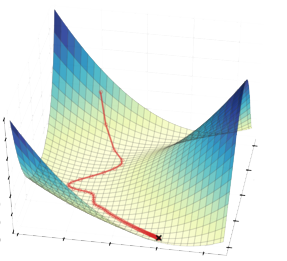
\includegraphics[width=\linewidth]{GD.png}
    \caption{Gradient Descent}
    \label{fig:my_label}
\end{figure}

Our main purpose is to find out a series of weight vectors (or a two dimensional weight) that minimize the total error on whole dataset. We implement Stochastic Gradient Descent (SGD)[12] as our learning method. The idea of Gradient descent (GD) is to update parameter along the gradient-descending direction. As shown in Figure 2, the red line shows that the total error decreased step by step from peak to bottom. Our purpose can be written as
\begin{equation}
    \arg \min_{\theta} J\left (\theta \right )
\end{equation}
However, one insufficient aspect of gradient descent is: in every iteration, the updating value depends on the gradient of all input,
\begin{equation}
    \theta_{c} = \theta{c} - \alpha \sum_{i}\bigtriangledown \left( w_{c}^{i}\cdot x^{i} - y\right)
\end{equation}
The stochastic gradient descent method randomly choose one direction of the gradient to descent, that is
\begin{equation}
    \theta_{c} = \theta{c} - \alpha  \bigtriangledown \left( w_{c}^{i}\cdot x^{i} - y\right)
\end{equation}
which means that the weight vector of a (conference, affiliation) pair will be updated after observed every input. The concrete update formula is 
\begin{equation}
    w_{c}^{i} = w_{c}^{i} - \alpha \frac{\partial J \left( \theta \right )}{\partial w_c^i},
\end{equation}
\begin{equation}
   \Rightarrow w_{c}^{i} = w_{c}^{i} - \alpha \frac{\partial J \left( \theta \right )}{\partial \hat{y}}\cdot \frac{\partial \hat{y}}{\partial w_c^i}
\end{equation}
\begin{equation}
   \Rightarrow w_{c}^{i} = w_{c}^{i} - \alpha \left( \left( \hat{y}-y\right)x_c^i + \lambda w_c^i\right)
\end{equation}
As shown in equation (13), in order to prevent the over-fitting problem in regression, we implemented a lambda regularization constant into our model. The regularization constant will change the updating step value in SGD. When lambda is small, the learning process will complete in few iterations while the accuracy on train set is far better than test set. Increasing the lambda constant will decrease the step length of each updating iteration which will finally slow down the learning process. However, a lambda too large turns out to be a bias on both train and test set which will increase the error on both train and test set.\\
In the training process of regression, we found that a large learning rate will lead to floating number overflow problems in python. The main reason is the input vector has not been normalized into the scale of (0,1). In that case, the gradient in each step is too large for the weight vector (our weight vector is initialized with zeros) so that the weight vector changed too sharply in each step. According to Figure 2, the total error will jump from one peak to another instead of decreasing along the path shown in the figure.

\subsection{Ensemble}
 Qian and Dong[7] implement ensemble model to enhance the overall performance but they were finally hindered by the ensemble model on some conferences. The ensemble method they used is to linearly combine the ranking score predicted by Ranking SVM and Regression. However, the actual rank is not linear to the ranking score. For example, if you double all the scores, you will get the same rank as before. Thus, we propose to ensemble models through results of ranking.
 
 \begin{table}[h]
 \centering
 \caption{Ensemble rank\newline}
 \begin{tabular}{c|c|c|c|c}
    \hline
      Affiliation& Method1& Method2& Ensembled &Result\\
    \hline 
      CMU&1&3&2&2\\
    \hline
      NEU&3&2&2.5&3\\
    \hline
      IBM&2&1&1.5&1\\
    \hline
 \end{tabular}
 \end{table}
As shown in Table 2, we combine the rank result from Method 1 and Method 2 to calculate a average ranking of an affiliation. After such combination, we re-rank affiliations. According to the ensembled rank in Table 2, the final result will be IBM@1,CMU@2,NEU@3. 

\section{EXPERIMENTS}
In this section, we elaborate on the empirical experiments we conducted to demonstrate the effectiveness of our improved model comparing with traditional model brought by the winner of KDD Cup 2016. Firstly, we will describe the specifics of the dataset recommended and provided by the competition organizer and how we make use of it. And then we visualize some of the experiments results through tables and charts. In the end, we discuss the underlying rationales of the improvements we made and the impact of dimensionality in feature engineering. Our source code of model implementations and extracted features are made publicly available on GitHub at [9].

\subsection{Experiment Setup}
We started with data processing and separated the responsibility of model implementations while using the same feature space. All implementation was written in Python scripts; the School-based Regression Model was completely written from scratch while the Ranking SVM utilized and modified Joachims' C++ implementation of $SVM^{rank}$[2].
We started with simple features and tried various ways of combining features. The algorithm we evaluate the performance of various model is the NDCG@20 (refer Introduction section).

\subsection{Data Processing}
We first parsed and imported the downloaded data-set text files into a SQLite database using Python. After relational design and indexing, the size of the database was able to maintain under 100GB. 
We then filtered and selected entries that are specific to our models. More specifically, entries that are from year 2011-2015, from all related conference shown in Table 1.
Since the dataset do not contain year 2016's end results, we use entries from year 2011-2013 as training set; 2014 as held-out set and 2015 as test set.
The selected data was later calculated into a feature space and stored as a hash map whose key is the Affiliation-Conference-Year triple as discussed in the Feature Engineering section. 

\subsection{Experiment Results}
 

%table1
\begin{table*}[h]
\centering\scriptsize
\caption{Performance of different method (NDCG@20)
\newline}
    \begin{tabular}{ccccccc}
    \hline
          & Conference& Baseline & Ranking SVM & Regression & School-based&Ensemble\\
    \hline
     
        &KDD& 0.7828& 0.9506& 0.9491&\textbf{0.9538}&0.9573\\
        &ICML& 0.8918& 0.8613& 0.8807& \textbf{0.9368}&0.8604\\
        &FSE& 0.5815& 0.6441& 0.6966&\textbf{0.8732}&0.6772\\
        &MobiCom& 0.6763& 0.6541& 0.6784&\textbf{0.8576}&0.5921\\
        &MM& 0.5331& 0.8412& 0.8405& \textbf{0.9148}&0.7563\\
        &SIGIR& 0.7664& 0.9022& 0.9219& \textbf{0.9711}&0.8939\\
        &SIGMOD& 0.7979& 0.8363& 0.8557& \textbf{0.9398}&0.8487\\
        &SIGCOMM&0.7788&0.8078& 0.8142& \textbf{0.8459}&0.6284\\
        &Average& 0.7261& 0.8149& 0.8910& \textbf{0.9267}& 0.7768\\
 
    \hline
\end{tabular}%
\end{table*}%


\begin{figure}[!h]
    \centering
    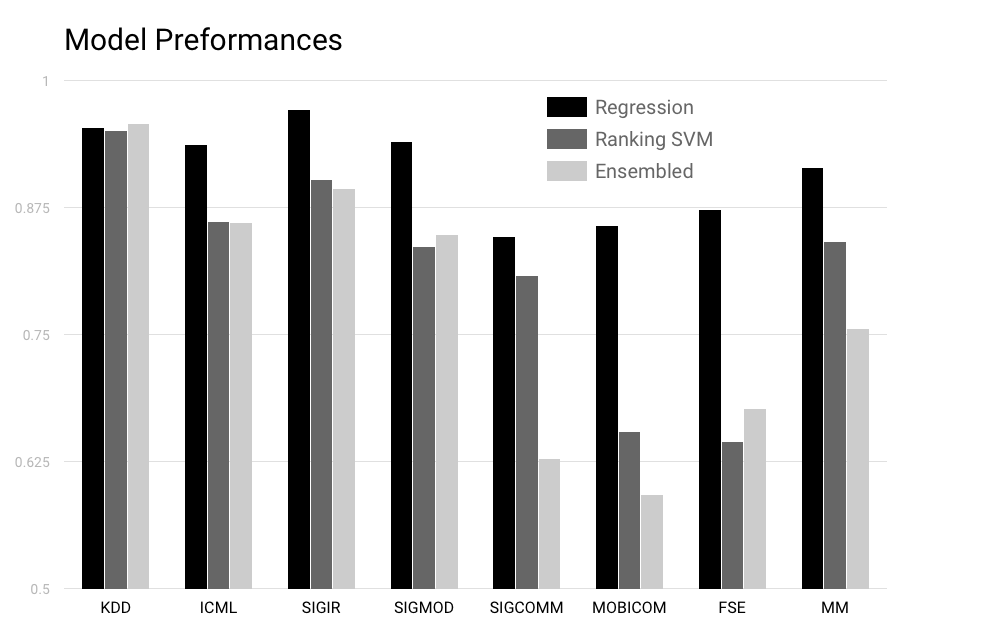
\includegraphics[width=10cm,height=6cm]{modelPerformace.png}
    \caption{Model Performance}
    \label{fig:my_label}
\end{figure}

%table4
\begin{table}[!h]
\centering\scriptsize
\caption{Average performance comparison of different feature engineering method(NDCG@20)
\newline}
    \begin{tabular}{ccccc}
    \hline
          & Method& Regression&School-based Regression\\
    \hline
        &Add& 0.8194& 0.9115\\
        &Average& 0.8206& 0.8993\\
        &Combine& 0.8170& 0.9100\\
    \hline
\end{tabular}%
\end{table}%

\begin{figure*}[!ht]
    \centering
    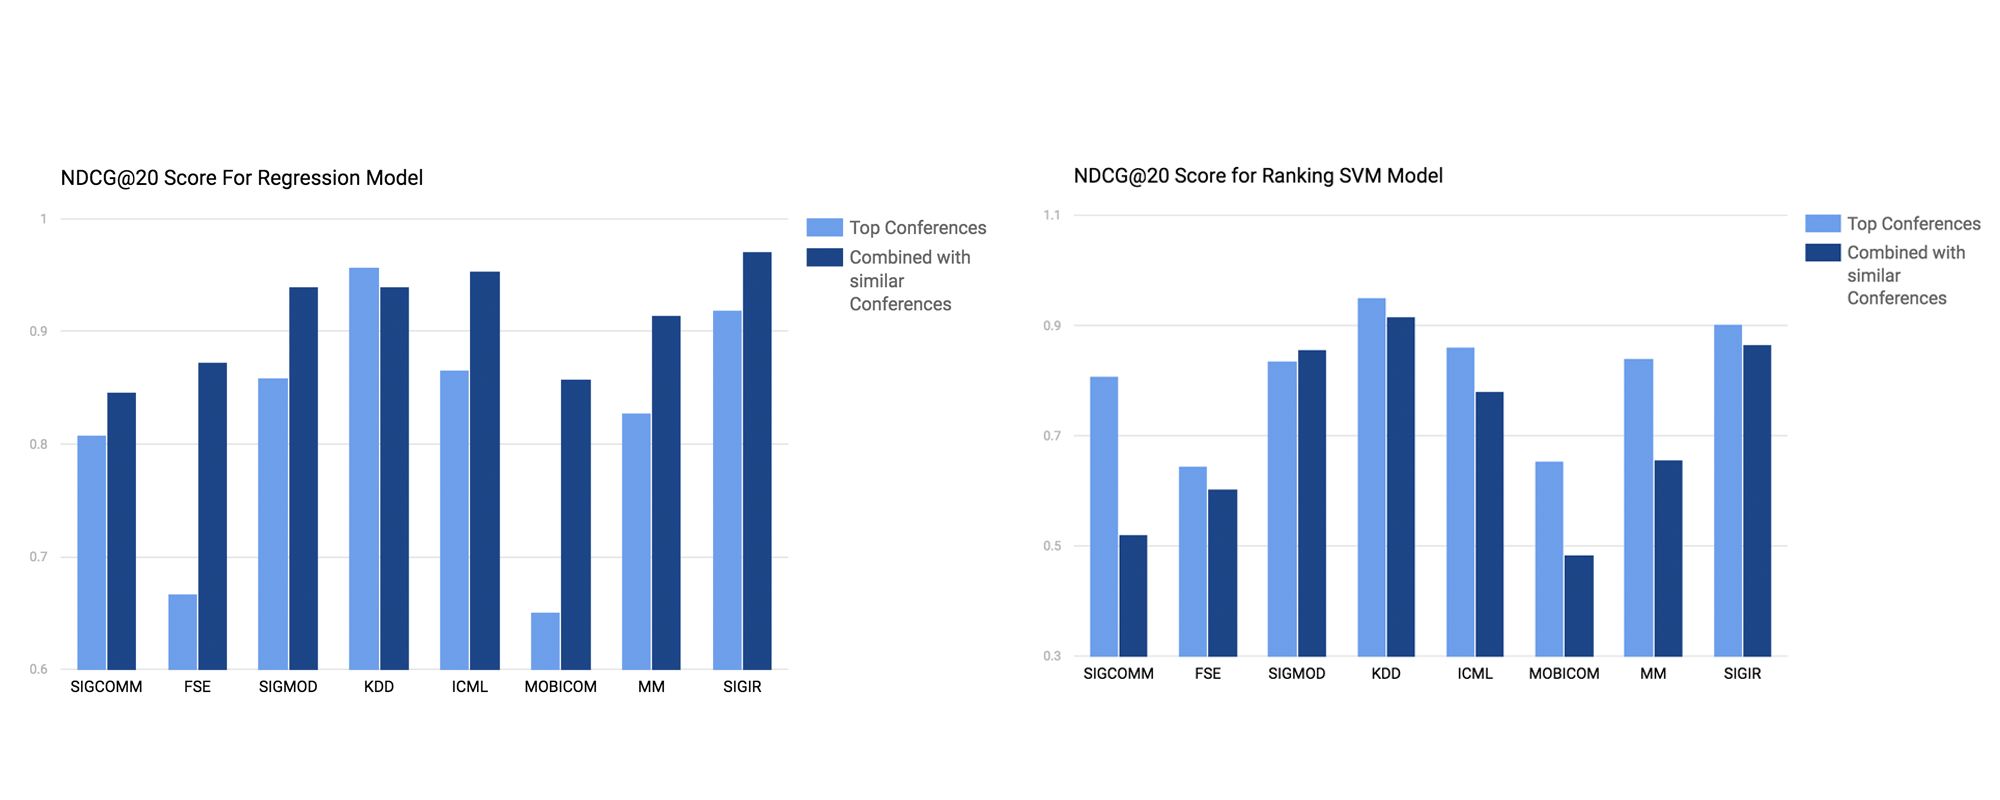
\includegraphics[width=\linewidth]{combined.png}
    \caption{Comparison of Ranking SVM and Regression}
    \label{fig:my_label}
\end{figure*}
As shown in Figure 3 that our School-based Regression Model out performed all other models including Ranking SVM model and even Ensemble Model. Note that School-based Regression model have a higher score comparing to traditional Regression model on all three ways of composing features (Table 4).

\subsection{Discussion}
From the results above, we observe that there are improvements and also discrepancies between what one would normally expect in terms of different ways of composing features.

\subsubsection{Why KDD perform the best?}
The performances of methods vary on different experiments settings. However, all methods perform well on KDD conference and SIGIR conference. We try to figure out the reason of this phenomenon by analyzing the input data. The top affiliations in these two conferences are comparably stabler than other conferences. Another reason why regression model that utilizes similar conferences information performs well on KDD and SIGIR is that the similar conferences of KDD and SIGIR are also top conferences in their field of study. For example, CMU published 4 paper in MobiCom while it published 0 paper in a similar conference of MobiCom. In which case, the information introduced into our model for this input instance is 0. Top affiliations which contribute their papers to KDD may also tend to send their works to these top conferences but not to those normal conferences. Thus, regression method outperforms on KDD and SIGIR than others because of involving more similar conferences information than other conferences.

\subsubsection{Information added by similar conferences}
As we can see in figure 4 that adding similar conference information in the features helps regression model to achieve almost better accuracy score on every conference. This increase in performance matches our expectation: enriched complexity helps the model to learn more and be closer to the ground truth. On the contrary, similar-conference information decreases accuracy for Ranking SVM model and we have not yet had valid hypotheses so that we purpose this problem to future research.

%table5
\begin{table}[htbp]
\centering\scriptsize
\caption{Performance comparison of using single conference and combination of relative conference(NDCG@20)}
    \begin{tabular}{ccccc}
    \hline
          & Method& Ranking SVM & School-Based Regression\\
    \hline
     
        &Single& 0.8123& 0.8195\\
        &Combined-input& 0.7104& 0.9117\\
    \hline
\end{tabular}%
\end{table}%

\subsubsection{Performance of Ensemble}
Unfortunately, our ensemble model also performs worse than regression as shown in Figure 3. We suppose that the main reason is that we use Ranking SVM whose NDCG@20 score is 10\% lower than regression as the ensemble sub-model. Thus, such combination actually weakens the good results from regression.
\section{CONCLUSION}
In this paper, we address a ranking problem designed by KDD Cup 2016 and are able to show that we improved Qian and Dong's Ensemble Model [7] which ranked 2nd overall in the competition by incorporating school information in the learned weights of our regression model.
In the meantime, we argue that the feature extraction process can be further improved by including citation and field of study information.  
We also showed that bringing similar conference information may or may not work well on different types of conference. 

\section{REFERENCES}

[1] T. Joachims, Training Linear SVMs in Linear Time, {\it Proceedings of the ACM Conference on Knowledge Discovery and Data Mining (KDD)}, 2006.\newline
[2] T. Joachims, Optimizing Search Engines Using Clickthrough Data, {\it Proceedings of the ACM Conference on Knowledge Discovery and Data Mining (KDD)}, ACM, 2002.\newline
[3] Vladimir N. Vapnik, {\it The Nature of Statistical Learning Theory. Springer}, 1995.
\newline
[4] Järvelin, Kalervo, and Jaana Kekäläinen. "Cumulated gain-based evaluation of IR techniques." {\it ACM Transactions on Information Systems} (TOIS) 20, no. 4 2002.\newline
[5]	Sinha, Arnab, et al. "An overview of microsoft academic service (mas) and applications." {\it Proceedings of the 24th International Conference on World Wide Web.} ACM, 2015.
\newline
[6] Sandulescu, Vlad, and Mihai Chiru. "Predicting the future relevance of research institutions-The winning solution of the KDD Cup 2016." {\it arXiv preprint arXiv}:1609.02728 (2016).
\newline
[7]Qian, Yujie, et al. "Feature Engineering and Ensemble Modeling for Paper Acceptance Rank Prediction." {\it arXiv preprint arXiv}:1611.04369 (2016).
\newline
[8] Wilson, Jobin, et al. "Ranking academic institutions on potential paper acceptance in upcoming conferences." {\it arXiv preprint arXiv}:1610.02828 (2016).
\newline
[9] Lu, Xueguang, and Diyi Wang. {\it University Ranking System. UniversityRankingSystem}. N.p., n.d. Web. https://github.com/xueguangl23/UniversityRankingSystem.
\newline
[10]Hastie, Trevor, Robert Tibshirani, and Jerome Friedman. "Boosting and additive trees." {\it The Elements of Statistical Learning.} Springer New York, 2009. 337-387.
\newline
[11]Box, George EP, et al. {\it Time series analysis: forecasting and control.} John Wiley \& Sons, 2015.
\newline
[12]Bottou, Léon. "Large-scale machine learning with stochastic gradient descent." {\it Proceedings of COMPSTAT'2010.} Physica-Verlag HD, 2010. 177-186.
\newline
[13]Hamilton, James Douglas. {\it Time series analysis.} Vol. 2. Princeton: Princeton university press, 1994.

\end{document}
